\graphicspath{{./}{./figures/}{./figures/synthexplore/}}

% Principle curve stuff could be neat
% \iffalse
% Other stuff to add:

% * 1d navigation
% * Principle curve: https://pypi.org/project/prinpy/ (https://web.stanford.edu/~hastie/Papers/Principal_Curves.pdf)
% \fi


\chapter{Designing an Exploratory Synthesizer Interface}
\label{chapter:synth-explore}

In this chapter the author introduces Synth Explorer: a prototype of an automatic synthesizer programming interface built on top of the torchsynth synthesizer described in the previous chapter. Synth Explorer is an interactive visual browsing interface for torchsynth that was built with the goal of supporting both novice and expert users in the process of navigating and developing an understanding of the vast and complex sonic space expressed by a synthesizer. It builds upon previous research in the area of sound visualization, and the design is informed by concepts from the the fields of creativity support tools (CSTs) and music interaction \cite{shneiderman2007creativity, holland2013music}. These concepts, along with the taxonomy of automatic synthesizer programming interaction approaches presented in \S\ref{chapter:asp-background} grounds the the development of Synth Explorer and provides a framework for the development of future systems. %Synth Explorer is an example of an exploratory interface, with potential for inclusion of additional interaction style, such as an example-based interface. I hope that this 

Synth Explorer is designed with music producers, audio practitioners, and synthesizer users in mind -- all individuals who regularly require synthesized sounds for their creative projects. Currently, users must manually program a sound, find an existing preset, or find a pre-existing sound in a collection of samples. Challenges with manually programming sounds is addressed in detail in chapter \S\ref{chapter:background}. Searching for presets and pre-existing sounds typically involves browsing through items that are displayed in a list-based user-interface. Any searching is based on filenames or semantic tagging \cite{knees2016searching}. In conversations held by Kristena Andersen at the RedBull Music Academy \cite{andersen2016conversations}, music producers expressed the challenges associated with navigating large collections of audio and their desires for improved methods for interaction. Particular emphasis was placed on the potential impact of tools that aid the creative process. The field of creative music information retrieval has also had the focus of finding ways to address the challenges of searching for sounds \cite{humphrey2013brief} and visual browsing interfaces have been identified as beneficial for allowing users to navigate large collections of sounds more efficiently than traditional list based methods \cite{turquois2016exploring}.

The interface implemented in Synth Explorer is intended to support the efficient navigation of synthesizer sounds, allowing users to develop a ``sound palette" for their project. Users are able to ``look under the hood" of the visual interface and directly interact with the underlying control interface for these sounds. They can make fine adjustments to the parameter settings to refine their selected sounds as well as to gain insight into the parameter settings that lead to the resulting sound. In this way, users can interact with the synthesis engine and control interface at a level abstraction that supports their position on the learning curve. The graphical interface is designed to support novice users. While the interface includes some technical audio terms, the drag and drop interface is modelled off of an interaction modality that will be familiar to most computer users and will allow anyone to quickly start constructing visualizations and exploring sounds. The inclusion of the technical names will allow users to begin to build up an understanding of the different dimensions of sound and how they relate to the underlying synthesizer parameters.

\section{Related Work}

Exploration-based interfaces for synthesizers was reviewed in chapter \S\ref{chapter:asp-background} and visualization of sounds based on sound similarity has been studied in depth and is reviewed by Cooper \textit{et al.} \cite{cooper2006visualization}. Within the field of automatic synthesizer programming, Synth Explorer is related to the data-driven approach used by in SynthAssist \cite{cartwright2014synthassist}; all the sounds used in Synth Explorer are pre-computed and audio features are stored in a database. Synth sounds are then displayed on the interface based on sound similarity. Looking beyond synthesizer sounds, work that is particularly relevant to Synth Explorer is DrumSpace, a 2D visualization interface developed by Turqois \textit{et al.} for exploring large collections of drum sounds \cite{turquois2016exploring}. A component of their study was a subjective evaluation that compared user experiences in browsing for drum sounds using a traditional list-based layout of samples to 2D visual layouts. For the 2D layouts they compared one method that automatically sorted sounds based on sound similarity against one that organized sounds based on the filename. Users reported having a significant preference for for the 2D based layout, but had no significant preference for the type of layout. Participants were able to explore a much larger number of audio examples in a shorter period of time when using the 2D interfaces. Turqois \textit{et al.} also identified that the layout based on sound similarity caused some confusion to the users; the layout was based on a set of audio features which had been reduced to 2D using a dimensionality reduction technique called t-SNE \cite{van2008visualizing}, because algorithms like t-SNE create complex combinations of higher dimensional features into a lower dimensional embedding for visualization, the meaning of the resulting dimensions used for visualization are often hard to identify. Turqois \textit{ et al.} also suggest that color could be a helpful addition to the interface. Building upon this work, the author of this thesis conducted further experiments on the perceptual relevance of different methods of dimensionality reduction techniques for visualizing drum samples in 2D and identified MDS as having the highest correlation with user similarity ranking \cite{shier2021manifold}. Synth Explorer builds on these tools and leverages similar techniques for creating 2D visualizations of synthesizer sounds.

An interesting CST that is related to the audio synthesis problem is a tool developed by Andrews for exploring and generating graphics using a 2D interface \cite{10.1145/3325480.3325506}. Their work used an algorithmic method for generating 2D graphics, which a user is able to interact with to control the generation of new graphics. Because of the vastness of the space of potential images that could be generated by the algorithm, the user interface utilizes a spatial layout of images to allow the user to quickly assess a set of possibilities which they can then use to guide the generation of further images. While this interface was focused on the generation of images, the interaction ideology is similar to that of Synth Explorer, which is built on top of an algorithmic audio synthesis engine; the space of possible sounds that a synthesizer can produce is far too vast for a user to navigate all at once, so a small random subset of that space is initially presented and the user is then able add more sounds and hone in on a particular result.

\section{Design Principles}
This section presents an overview of design principles, informed by the HCI fields of music interaction and creativity support, that are intended to guide the development of automatic synthesizer programming interfaces. These principles provide a framework for designing interactions from the perspective that a synthesizer is a musical tool that users \textit{want} to engage with in the context of a creative pursuit -- whether that is designing sounds for a film soundtrack, composing a piece of electronic music, or simply enjoying creating sounds and playing a synthesizer. Because of the breadth of what a creative pursuit can encompass, these principles are intended to be taken as suggestions to help situate the design process.

\subsection{Music Interaction}
Music and Human-Computer Interaction \cite{holland2013music}, or simply Music Interaction, is the field of research related to the use of interactive systems that involve computers for any kind of musical activity. Music interaction not only draws heavily from other areas of HCI research, but also responds to the needs and desires of the music community. There are unique considerations that make music interaction different from other fields of HCI. A musical instrument is not a utilitarian tool whose development should be ever-improved and made more efficient. Musical instruments are played; sometimes that is the only goal. Tanaka \cite{tanaka2000musical} identifies that imperfections and limitations of a musical instrument give an instrument character. This was reflected by music producers interviewed by Andersen who expressed the role of serendipity and ``happy accidents" in their creative process \cite{andersen2016conversations}, and identified this as an important consideration for designing new music production tools. McDermott \cite{mcdermott2013should} identifies the importance of engagement in musical interaction and the relation that bears to the concept of \textit{flow}. Mihaly Csikszentmihalyi coined the term \textit{flow} to describe a state of highly focused concentration that is related to experiencing an activity as being deeply satisfying and engaging \cite{csikszentmihalyi1990flow}. The role that the learning curve plays is crucial to the level of engagement that a player experiences when playing a musical instrument, both in the short-term and the long-term. Holland \cite{holland2013music} concludes, ``In order to remain engaging, consuming and flow-like, activities that involve musical instruments must offer continued challenges at appropriate levels of difficulty: not too difficult, and not too easy." 

Automatic synthesizer programming tools can be thought of as being extensions of a musical instrument. With this in mind, the goal should not necessarily be to provide a perfectly optimized experience that completely takes over the task of programming and using a synthesizer. For example, example-based inverse synthesis approaches may play an important role in an automatic synthesizer programming tool; however, they may only be one part of a larger interaction paradigm that provides other opportunities for expression. The inclusion of design features that allow for ``happy accidents" to occur and unexpected use-cases to be realized can lead to more engaging and rewarding experiences. In fact, there is a rich history in music technology of musicians using devices in an \textit{incorrect} way with great success. The Roland TB-303 is an excellent example of this: the synthesizer failed at a its initial goal of generating realistic bass sounds. However, its synthetic ``squelchy" tones resulted in it leading a successful second life as an electronic dance music instrument \cite{vine2011tb303}. It is impossible to design an interface with the unexpected use in mind; however, leaving enough room for features to be used in unexpected ways is a method to encourage long-term engagement. In addition, related to the concept of engagement is the consideration of the role that the learning curve plays while using a synthesizer. Building in interactions that support users as they progress along the learning curve will also encourage both short-term and long-term engagement.

\subsection{Creativity Support}
Related to music interaction is the study of creativity support tools. Design guidelines borne out of research in creativity support tools is relevant to the design of tools that support synthesizer users. Shneiderman \cite{shneiderman2007creativity} outlines a set of design principles for developing creativity support tools which include the following: support exploratory search; enable collaboration; provide rich history keeping; and design with low thresholds, high ceilings, and wide walls. Davis \textit{et al.} focus on the role that CSTs play in supporting novices engaging in creative tasks and the relationship that the environment plays in creativity \cite{davis2013toward}. In their work, the authors identify two types of novice users: domain novices and tool novices. Domain novices are new to both the creative domain as well as using the creativity support tool. Tool novices have experience with the creative domain, but are novices at using a particular tool. To help evaluate and promote the development of creativity support tools for novices, they also propose a theory of creativity support based on three cognitive theories: embodied creativity, situated creativity, and distributed creativity.

\textbf{Embodied creativity} is based on the premise that creativity is intrinsically linked to the interaction that a user has with their environment. It is through interacting with their world that an individual is able to make creative ideas more concrete and express themselves. In chapter \S\ref{chapter:asp-background} I reviewed the various approaches to automatic synthesizer programming, which included six different interaction paradigms: evaluation interfaces, use of descriptive words, vocal imitations, exploration interfaces, example-based interfaces, and intuitive controls. These represent some of the ways in which a system might support a user in expressing and developing their creative ideas when using a synthesizer. An interaction may including one or more these paradigms, but is not limited to this specific set of interactions.

\textbf{Situated creativity} is related to the concept of flow. In the context of creativity support, situated creativity is linked to how much effort a user must apply when using a tool to carry out a task. As a user becomes more comfortable with a tool, it gradually starts to feel like a natural extension of their body and they are enabled to explore deeper expression of their creativity. This is related to the learning curve and level of engagement that a musical interaction is able to support, which is discussed in the previous section.

\textbf{Distributed creativity} is focused on the tasks that a human can offload to a particular tool during a creative task. By handing over a portion of a creative task to a support tool, a novice user may be able to arrive at rewarding results earlier in the process, thereby motivating them to continue to engage in the creative process and enhance their skills. A large portion of the previous work in automatic synthesizer programming has been dedicated to the development of algorithms that automate the task of programming a particular sound in a synthesizer. These methods provide opportunities for distributing the creative load, especially to help novice users who are at early stages of the learning curve.

\section{Synth Explorer Design}
Synth Explorer is designed to support exploration and provide a low threshold of entry for users to begin working with synthesized sounds within a creative context. It is an exploration-based interface that overlays a synthesizer and provides a visual representation of sounds generated by that synthesizer. The visual interface is aimed at tool novices \cite{davis2013toward}: users who may have expertise in composing music and working with digital audio workstations, but may have limited experience in working with audio synthesizers. To support progression along the learning curve, users are able to explore and adjust the underlying synthesizer parameter settings for any sound to help them develop their understanding of programming.

Synth Explorer is expected to be an accessory tool used during the creative process of composing digital music in addition to a users' main digital audio workstation. For example, a user might be composing a film soundtrack in their workstation of choice and find that they are desiring to add a new synthesized instrument to their score. In this example, the user would open up Synth Explorer, browse for a sound that fits their needs, and then load those sounds back into their workstation. While navigating between two different programs may seem like an impediment to the creative flow, it is hypothesized that the added benefits of the Synth Explorer interface will outweigh the inconvenience of switching between programs. Additionally, future iterations of the tool could be implemented as a VST plugins as well as host VST synthesizer plugins to support better integration with current music production processes.

The user interaction methodology was designed according to the theories of cognition presented by Davis \textit{et al.} for supporting novice users working with CSTs: embodied creativity, situated creativity, and distributed creativity \cite{davis2013toward}. The design of Synth Explorer in relation to these three aspects is presented below.

\subsubsection{Embodied Creativity}
The browsing interface should support embodied creativity -- the layout and interaction with the browsing interface should use multiple modes of sensory cognition to facilitate understanding. Spatialization of multimedia objects based on similarity has been used in previous related work \cite{10.1145/3325480.3325506} and is used here to provide deeper insight into the relationship between sounds. Based on the previous issues identified with 2D visualizations of sound, which caused confusion to users \cite{turquois2016exploring}, the user here is given control over how the visualization is constructed to empower them to develop an understanding of the spatial relationship between sounds. Specifically, users are able to assign audio features to the x, y, and color of each sound object on the 2D layout.

\subsubsection{Situated Creativity}
Synth Explorer should support a user in maintaining creative flow while working on their project. Additionally, the user interface should have a low threshold of entry to enable novices to quickly start engaging with sounds and working towards realizing their creative goal. The conscious effort required to use Synth Explorer should quickly dissipate into the subconscious, allowing the user to instead focus the entirety of their attention on the creative task at hand. At the same time, Synth Explorer should implement features that support longer-term engagement by challenging users as they progress along the synthesizer programming learning curve. The visual exploration interface is intended to support short-term engagement aimed at novice users -- while still remaining enjoyable for more experienced users -- and to support more depth and longer-term engagement through allowing users to modify synthesizer parameters directly on a separate interface.

\subsubsection{Distributed Creativity}
Synth Explorer should offload the laborious task of organizing large collections of sounds and navigating the sonic space represented by a particular synthesizer. The system should also not take full control over the creative process and provide the user with room to express creative control. In a traditional synthesizer, a user would need to learn how to program sounds themselves, rely on experts to create and organize presets, or organize presets themselves. Applying distributed creativity to Synth Explorer, the user should offload the task of programming and organizing synth presets over to the system and shift their energy to the task of curating a selection of sounds that fit the needs of their creative vision.

\section{Implementation}
\subsection{Sound Generation and 2D Mapping}
The core of Synth Explorer is the synthesizer. The torchsynth synthesizer introduced in \S\ref{section:torchsynth} was used for this prototype system. The default \textit{Voice} architecture for torchsynth was used, which is a basic two oscillator + noise synthesizer with multiple modulation sources and a modulatable amplifier. Sounds are generated from a subset of the synth1B1 dataset (see \S\ref{section:synth1B1}) and the resulting four second audio clips and parameter settings are saved. Audio features are computed on each audio clip and the dimensionality reduced in order to visualize these sounds in two dimensions based on sound.

Audio features are designed to capture perceptually relevant aspects of audio in a compact format. In DrumSpace, the 2D visualization of samples was produced by computing a set of audio features and then performing dimensionality reduction to two-dimensions using t-SNE \cite{turquois2016exploring, van2008visualizing}. In subsequent work, the UMAP dimensionality reduction algorithm \cite{mcinnes2020umap} was found to be an effective alternative to t-SNE in terms of time-complexity and visualization quality \cite{jiale2020visualization}. Synth Explorer uses two different UMAP embeddings as options for visualization: an embedding based on mel-frequency cepstral coefficients and an embedding based on spectral features \cite{peeters2004large}. In addition to these dimensionality reduced embeddings, a set of eight low-level audio features computed using librosa\footnote{\url{https://librosa.org/doc/latest/index.html}} are included. In addition to audio features, parameter values are also included as features that can be visualized. This supports users in beginning to build up an understanding of the complex relationship between the parameter space and auditory space. The parameter setting (preset) for each sound comprises 78 individual parameter values. UMAP embeddings are computed on the parameter settings to create two dimensional parameter features for visualization. Additionally, the keyboard pitch is included.
% TODO if time.
%[Include a table of the full list of available features]

The database of audio files and associated features allows the synthesizer sound space to be automatically organized based on these features. This addresses the distributed creativity component of the design. The user offloads the task of generating synthesizer sounds and organizing them to the system. Due to the speed of the synthesis system and audio feature extraction process, nearly ten thousand unique sounds can be generated and analyzed in about 20 minutes. This corresponds to over ten hours of synthesized audio. Listening to and organizing all these sounds would be impractical -- or at least extremely mundane -- for any user, whether they are a novice or expert. 

\subsection{Browsing Interface}

Using the guiding cognitive theories for developing creativity support tools, an interface was designed based on the aforementioned related work. A drag and drop interface, which is an interaction paradigm common to consumer computer user interfaces, is employed, that allows users to assign different features to the dimensions of the visualization. Instead of forcing a layout on the end user, the user has the ability to decide which feature / embedding they want to use to construct their visualization. This decision was made based on participant feedback that they were confused by the sound similarity visualization used in DrumSpace \cite{turquois2016exploring}. An attempt is made to address this issue by explicitly providing the user with a set of features ranging from concrete (keyboard pitch) to more abstract (spectral embedding using UMAP), and allowing them to decide which they want to use to create the visualization. Additionally, tooltips are provided for each feature which provides an opportunity for the user to learn more about the underlying dimensions and their relationship to audio perception.

The final interface is shown in figure \ref{fig:ui_1}. % include piece on embodied creativity and situated creativity
The workflow of the interface is divided into four different sections: adding sounds, constructing the visualization, exploring and saving sounds, and downloading saved sounds. An overview of each step in the workflow is provided in the following sections.
\vspace{1cm}
\begin{figure}[ht]
    \centering
    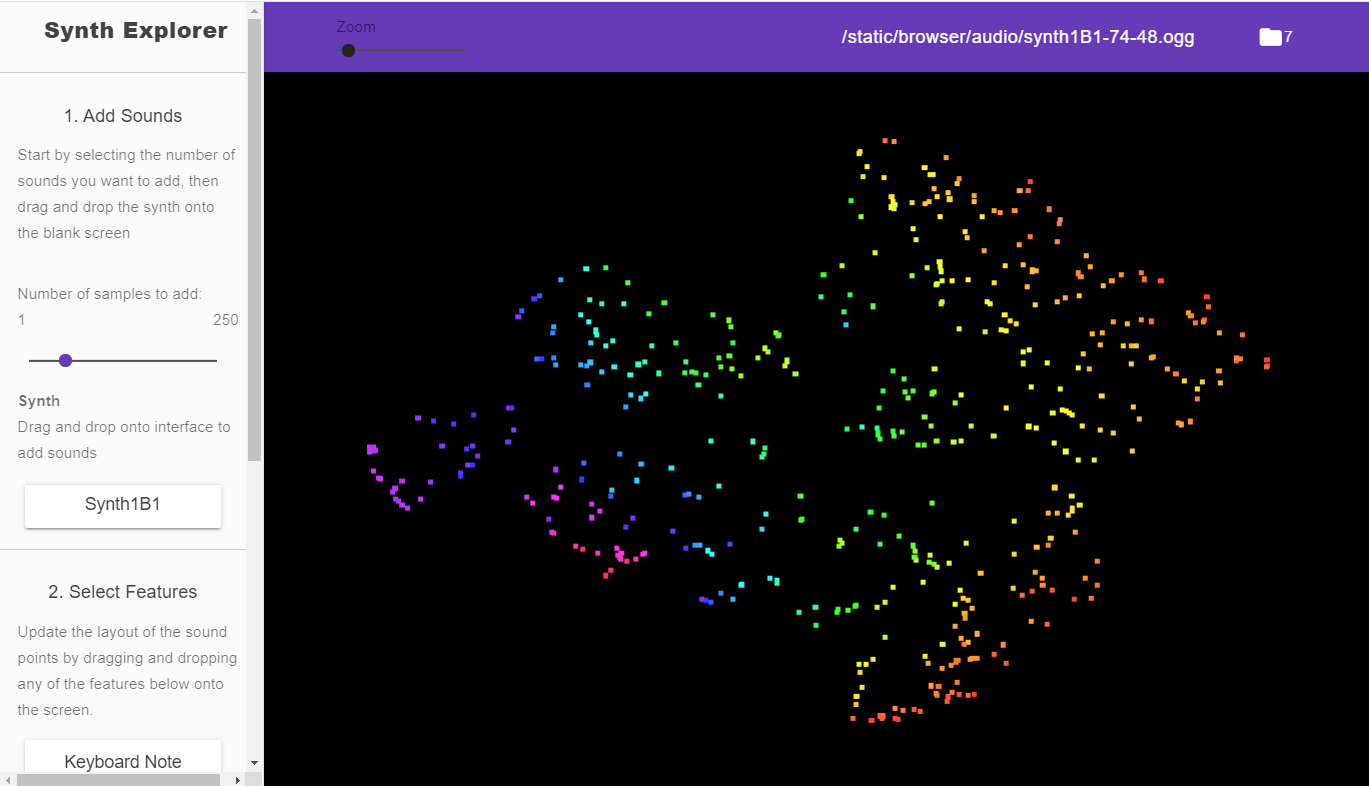
\includegraphics[width=0.8\textwidth]{SynthExplore Init.png}
    \caption{Synth Explorer User Interface}
    \label{fig:ui_1}
\end{figure}

\subsubsection{Adding Sounds}
The space of possible sounds that can be produced by a synthesizer is vast. Ten thousand four second audio clips of patches from \textit{torchsynth} represents only a subset of the possible sounds that torchsynth is capable of producing. That being said, presenting a user with ten thousand audio clips on a 2D layout would be overwhelming. The user is initially presented with a small random subset of possible outcomes. The user is given the option to control how many sounds are added to the visualization at once using a slider control that ranges between 1 and 250. They are then able to add that many sounds to the their visualization by dragging and dropping the UI object representing a particular synthesizer onto the visualization area. In this way, they can explore the sound space in an iterative fashion. This section of the user interface is shown in figure \ref{fig:steup 1}. Currently only one synthesizer is shown in the interface; however, any number could be included. This would allow the user to compare and explore multiple synthesizers at any given time. 

Once a user drops a synthesizer onto the visualization, the requested number of synthesizer sounds are randomly selected from the database and added to the interface. A single sound is represented as a single point on the 2D visualization.

\begin{figure}
    \centering
    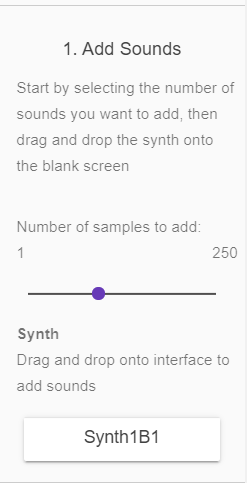
\includegraphics[width=0.2\linewidth]{SynthExplore_AddSounds.png}
    \caption{Synth Explorer Step 1}
    \label{fig:steup 1}
\end{figure}

\subsubsection{Constructing the visualization}
The next section of the user interface is focused on allowing the user to control their visualization. Specifically, this section allows users to decide which features are assigned to which dimension of the visualization. The available features are shown on the left side of the user interface in figure \ref{fig:features}. Using the same drag and drop paradigm, the user is able to drag any of the features onto the visualization surface in order to modify the layout of audio samples. When the user initiates a drag and drop interaction, large drop areas representing the different dimensions of the visualization appear for the user to choose from. The available dimensions are the x-axis, y-axis, and the color of the points. Once a feature is dropped onto one of the dimensions of the visualization, the points representing the sounds automatically shift into the new position to reflect the changes. Any feature can be associated with any dimension, allowing the user to explore the relationship between the features and develop a visualization that meets their needs.

A decision was made to use the technical names of the features. While this may be confusing to some users, there are unfortunately not many good alternatives to this problem. Tooltips are provided to give novices an approximate non-technical description of the feature -- the hope is that these users will still feel inspired to explore these different features and learn how they relate to the auditory dimensions of sounds.

\begin{figure*}
    \centering
    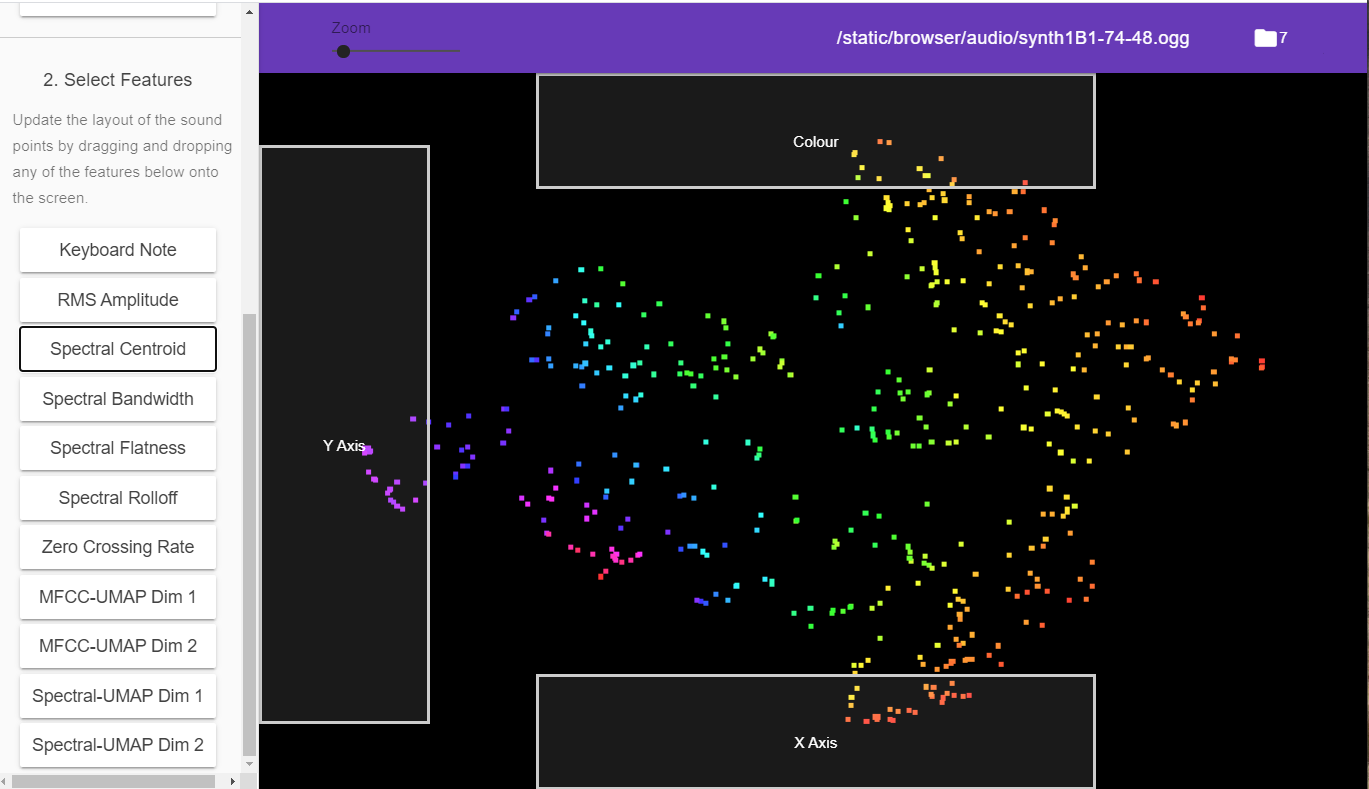
\includegraphics[width=0.9\textwidth]{SynthExplore A.png}
    \caption{Synth Explorer UI: Updating features}
    \label{fig:features}
\end{figure*}


\subsubsection{Exploring and Saving Sounds}
The majority of the space on the user interface is occupied by the 2D browsing space, which is shown in figure 2. This is the space where synthesizer sounds are represented as points on a scatter plot. To listen to a particular sound, the user simply hovers their cursor over the point representing a sound. They receive both auditory and visual feedback once they intersect with a point. The sound represented by the point plays and a small circle burst the same color as the point is animated into view at the point of interaction. Users can also zoom into the visualization using their mouse scroll wheel and navigate the space using a click and drag operation. Each of these gestures is meant to reflect operations that would feel intuitive and natural to an experienced computer user.

This mode of interaction provides a fast way for the user to preview a large number of samples. The goal of the 2D layout and exploration method is to provide the user with an embodied method for exploring sounds. The 2D spatial layout using colors provides users with a visual representation of the sonic space that they can interact with and create their own associations with. The interaction itself is easy to master as it simply requires dragging a mouse around the screen and listening to sounds. Modifying the layout using drag and drop interactions also requires little conscious effort. These intuitive interactions were implemented to support situated creativity and thereby aid creative flow.

When a user has listened to a sound that they like and want to save, they can press the ``s" key on their keyboard to save that clip to a ``sound palette". This is equivalent to adding an item to an online shopping cart. The user can then continue to explore sounds.

At this point the user is able to repeat any of the preceding steps and to continue explore the visualization: add more sounds, modify the dimensions with different features, explore the space, adjust parameters for a specific sound, and then save the resulting sounds.

\subsubsection{Adjusting Parameters}
At any point during exploration users can move to a secondary interface and work directly with the synthesizer parameters. This interface, shown in figure \ref{fig:adjusting-parameters}, is essentially a regular control interface for the torchsynth synthesizer that contains slider controls to update the values for all 78 of the parameters in the torchsynth Voice. These 78 parameters are grouped by the specific module that they control (see \ref{fig:voice_diagram} for a diagram of all the modules in Voice). When navigating to this screen, the parameter settings for the sound that was selected from the visual exploration interface will be showing; this allows the user to gain insight into the specific parameter values for that particular sound, as well as to make modifications on the sound.

\begin{figure}[ht]
    \centering
    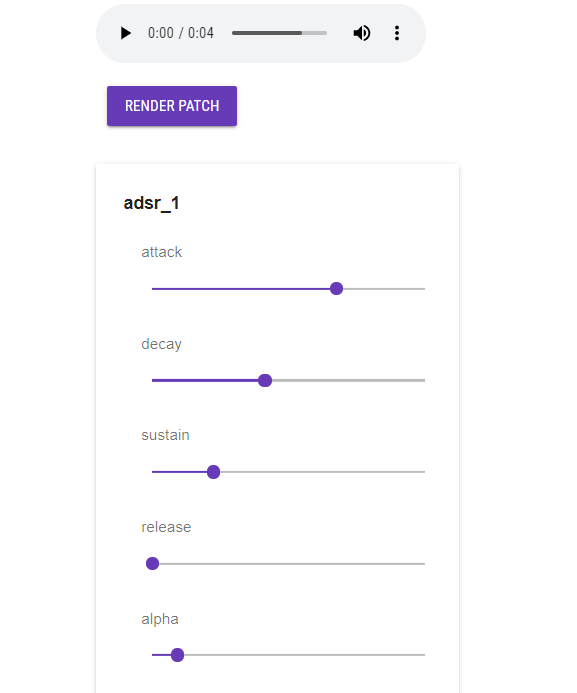
\includegraphics[width=0.45\textwidth]{figures/synthexplore/SynthExplore-Adjust-Param-Cropped.png}
    \caption{Interface for adjusting the parameter values for a synthesizer patch, allowing for fine-tuning of sounds found on the visual exploration interface }
    \label{fig:adjusting-parameters}
\end{figure}

\subsubsection{Downloading}
Once the user has sufficiently explored the sonic space and saved a palette of sounds they would like to use, they can click on the download icon next to their saved sounds and download all the synthesizer sound files they have saved. Once they have done this they are free to use those sounds for whatever creative task they would like.

\subsection{Technical Implementation Details}
Synth Explorer is implemented as a web application. The Django framework\footnote{\url{https://www.djangoproject.com/}} was used to implement the backend of the web app. Django is written in python and provides an elegant data-model system for interacting with a database such as MySQL\footnote{{https://www.mysql.com/}}. The sound generation and analysis portion of the application is written as a Django management command -- when this command is run, a set of sounds is rendered using \textit{torchsynth}, and analyzed using librosa and UMAP. Once the samples have been analyzed and audio files saved to disk, the audio features and patch settings for each sound is saved in a MySQL database.

The frontend of the application is written using HTML, CSS, and JavaScript. The foundation of the application was based on code developed by Leon Feddden \footnote{\url{https://github.com/fedden/umap_tsne_embedding_visualiser}}. This code was modified to function within the Django framework and the user interaction paradigm was modified to support dynamic adding of synthesizer samples and user construction of the layout using drag and drop interactions. The visualization and animation is rendered using three.js\footnote{\url{https://threejs.org/}}.

\section{Evaluation}
\subsection{Creativity Support Index}
The creativity support index (CSI) \cite{cherry2014quantifying} is a psychometric survey that was designed to quantify the ability of a tool to assist a user with a creative task. The CSI evaluates a creativity support tool based on six different criteria: Exploration, Expressiveness, Immersion, Enjoyment, Results Worth Effort, and Collaboration. The CSI is structured as a questionnaire with two different sections. The first sections contains 12 questions, shown in figure \ref{fig:csi}, which participants answer with a score from 1-10 (``Highly Disagree" to ``Highly Agree"). The second section contains 15 questions which compares each of the evaluation criteria pairwise and asks the participant the evaluate which criteria was better supported. For example, each question begins with “When doing this task, it’s most important that I’m able to...” followed by a two statements, where one statement is related to one of the evaluation criteria and the other is related to another. Participants are asked to select only one of the statements and each evaluation criteria is ranked against all the others. Based on the scores for these questions a CST is given a score out of 100. Synth Explorer was evaluated informally on two separate tasks that were designed to replicate a typical synthesizer use case in the context of music production.

\begin{figure}[ht]
    \centering
    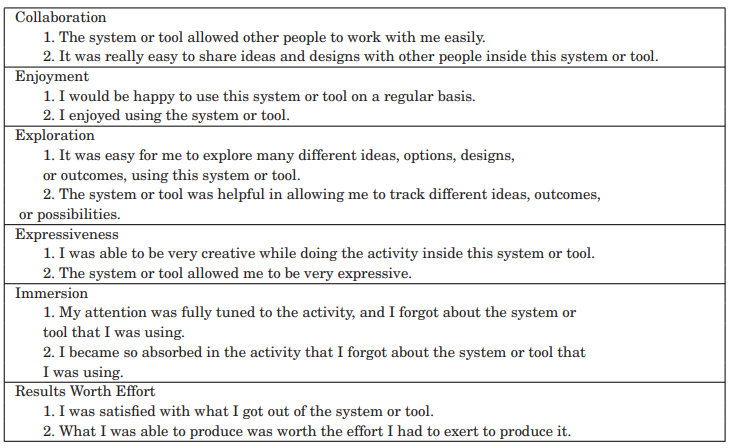
\includegraphics[width=0.99\textwidth]{figures/synthexplore/CSI-Questions.png}
    \caption{Agreement questions for the creativity support index}
    \label{fig:csi}
\end{figure}

\subsubsection{Task 1: Synthesizer browsing for an existing project}
In this task, the user is working on an existing musical project in a separate workstation. They are composing a piece of music and then are asked to find a new synthesizer sound for an additional track to their composition. They must leave the workstation,
open Synth Explorer, browse for a new sound, then leave Synth Explorer and open the new sound back in the workstation they were initially working within.

\subsubsection{Task 2: Creating a sound palette for a new project}
In this task the user is beginning a new project and is searching for a set of synthesizer sounds to create the sonic palette for the new composition. They may have a particular sound in mind, but they are asked to explore the interface in an open-minded way to look for new sounds and create a collection as inspiration to start the new project.

\subsection{CSI Results}
Results of the CSI evaluation are shown in table \ref{table:csi}. These results show that Synth Explorer supported task 1 to a greater degree than task 2. Task 1 received an overall score of 78.67 whereas task 2 received an overall score of 71.67. The results showed that collaboration was not supported and received a score of zero for both tasks. This makes sense considering the nature of the tasks and the tool itself. Collaboration was not a part of the evaluated tasks. However, the tool itself does not currently support collaboration in any meaningful way other than allowing two users to sit next to each other and browse for synth sounds simultaneously. The tool supported exploration in both tasks more than any of the other attributes evaluated. This result is positive considering that was one of the major goals for the tool. Another area that was well supported by the tool is enjoyment, while the results and expressiveness of the tool itself were not highly rated. The lack of expressiveness also makes sense for the tool; Synth Explorer itself does not necessarily allow expression -- it allows a user to explore sounds with the goal of maintaining a creative flow in a large creative context, despite it being more challenging to be expressive with the tool.

The results section of the evaluation did not score highly either. This was due to the fact that the 2D layout of sounds was still challenging to navigate and make sense of for users. This is in part due to the underlying method for generating sounds as well as the sound mapping techniques. Randomly sampling a synthesizer is not the best way to capture meaningful sounds from the synthesizer and a lot of times produces dramatic or unusable results. Additionally, capturing sound similarity in two dimensions is still an open question that requires further work. Despite this, the interface was effective at enabling rapid exploration of a large number of sounds and it was enjoyable getting to explore manipulating the visualization by dragging and dropping the different features onto the plot.

\begin{table}[th]
\centering
\begin{tabular}{l|llll|ll}
Area           & Q1 & Q2 & T1 & T2 & T1 Total   & T2 Total \\
\hline
Collaboration  & 1  & 1  & 0            & 0            & 0              & 0            \\
Enjoyment      & 7  & 8  & 5            & 4            & 75             & 60           \\
Exploration    & 10 & 7  & 5            & 5            & 85             & 85           \\
Expressiveness & 5  & 4  & 1            & 2            & 9              & 18           \\
Immersion      & 8  & 7  & 3            & 2            & 45             & 30           \\
Results        & 5  & 6  & 2            & 2            & 22             & 22           \\
Total Score    &    &    &              &              & \textbf{78.67} & \textbf{71.67} 
\end{tabular}
\caption{Results of creativity support index questionnaire.}
\label{table:csi}
\end{table}

\section{Future Work and Conclusion}
This chapter has introduced the Synth Explorer creativity support tool. The intention of this tool is to support users in the process of working with synthesizers and finding new sounds for creative projects. The development of Synth Explorer was based on a set of design principles informed by the fields of music interaction and creativity support tools. A further goal of the tool is to support novice users who might have experience in music production, but do not have experience working with synthesizers. Synth Explorer was designed to support novices using an approach to creativity support based on cognitive theory which emphasizes embodied, situated, and distributed creativity. The designed tool uses a 2D visualization of synthesizer sounds to arrange sounds spatially and uses colors to support an embodied approach to exploration. By using a simple drag and drop interface and browsing of sounds using a visual layout, users are able to quickly start exploring and remain engaged in their creative task. A secondary interface containing the individual parameter values allows users to engage in manual synthesizer programming using a sound from the visual interface as a starting point. This encourages long-term engagement through the inclusion of a more challenging interaction paradigm that provides a user with more depth of control.

An evaluation of the tool using the creativity support index revealed insight into the strengths and weaknesses of the tool and helped to identify areas for potential further work. The most glaring limitation of the tool is that it lacks support for collaboration; however, collaboration support could be added relatively easily based on the implementation. Since Synth Explorer is built as a web application using the Django framework, a user login system could be easily added to allow users to save and share collections of sounds that they have curated. Different synthesizers and layouts could also be shared through a similar system. Another limitation of the current system is in the available options to filter and search for sounds. Currently, users are limited to adding random samples to the interface and exploring different configurations of that. In order to support users in arriving at more useful results and collections of sounds, future iterations could provide additional search options, such as a search by similarity, or additional tools for selecting and filtering the current selection. Integrating more advanced sound searching methods, such as an example-based interaction paradigm using one of the approaches discussed in \S\ref{chapter:inverse_synth_experiment}, would also benefit future development. Providing support for playing the sounds using a real-time keyboard interface could also encourage more engagement and help the tool feel more like an extension of a musical instrument.